\chapter{Additional and related research involving evidence evaluation, biomedical knowledge graphs, and pharmaceutical discovery}

\section{CARLSBAD: Confederated, annotated research library of small-molecule bioactivity data}

CARLSBAD: Confederated annotated research library of small-molecule bioactivity data
The CARLSBAD Database: A Confederated Database of Chemical Bioactivities, S.L. Mathias et al., Database, 2013\cite{Mathias2013-hj}.

Integrated, chemically intelligent bioactivity knowledge graph

\subsection{Abstract}

Many bioactivity databases offer information regarding the biological activity of small molecules on protein targets. Information in these databases is often hard to resolve with certainty because of subsetting different data in a variety of formats; use of different bioactivity metrics; use of different identifiers for chemicals and proteins; and having to access different query interfaces, respectively. Given the multitude of data sources, interfaces and standards, it is challenging to gather relevant facts and make appropriate connections and decisions regarding chemical–protein associations. The CARLSBAD database has been developed as an integrated resource, focused on high-quality subsets from several bioactivity databases, which are aggregated and presented in a uniform manner, suitable for the study of the relationships between small molecules and targets. In contrast to data collection resources, CARLSBAD provides a single normalized activity value of a given type for each unique chemical–protein target pair. Two types of scaffold perception methods have been implemented and are available for datamining: HierS (hierarchical scaffolds) and MCES (maximum common edge subgraph). The 2012 release of CARLSBAD contains 439 985 unique chemical structures, mapped onto 1,420 889 unique bioactivities, and annotated with 277,140 HierS scaffolds and 54,135 MCES chemical patterns, respectively. Of the 890,323 unique structure–target pairs curated in CARLSBAD, 13.95\% are aggregated from multiple structure–target values: 94,975 are aggregated from two bioactivities, 14,544 from three, 7930 from four and 2214 have five bioactivities, respectively. CARLSBAD captures bioactivities and tags for 1435 unique chemical structures of active pharmaceutical ingredients (i.e. ‘drugs’). CARLSBAD processing resulted in a net 17.3\% data reduction for chemicals, 34.3\% reduction for bioactivities, 23\% reduction for HierS and 25\% reduction for MCES, respectively. The CARLSBAD database supports a knowledge mining system that provides non-specialists with novel integrative ways of exploring chemical biology space to facilitate knowledge mining in drug discovery and repurposing.

\subsection{Introduction}

As the number of chemicals and screening efforts multiply, the number of bioactivity databases offering information on biological activity of small molecules is increasing. They represent a rich source of information in our quest to map the chemical space of bioactive molecules to phenotypic and target space. We estimate that the space of publicly available bioactivity data indexes over at least 1.15 million unique chemicals, annotated onto \textgreater 15,000 targets\cite{Kim_Kjaerulff2013-hi}, with potentially an equal number of phenotypic screens. The exact magnitude of this space could be derived only if one could uniformly process these data into a single database and harmonize chemicals, targets, bioassays and bioactivities. Each of the many sources and databases available has its own interface and data query style, with both strengths and weaknesses. Such multitude of sources, interfaces and styles is likely to make it difficult for scientists who are not expert in data mining to gather all facts, make connections and appropriate decisions that would lead their own research to the best possible outcome.

This difficulty is best illustrated by considering the chemical biology of estrogen: estrogen-related macromolecular targets include at least five nuclear receptors (estrogen receptors $ER\alpha$ and $ER\beta$; estrogen-related receptors: $ERR\alpha$, $ERR\beta$ and $ERR\gamma$), one G-protein coupled receptor (G-protein estrogen receptor, or GPR30), aromatase, several sulfotransferases and sulfatases, as well as the sex hormone steroid-binding globulins. All these targets are associated with and recognize a common chemical pattern (CCP), namely, a para-substituted phenol at the 'A' ring. Non-steroidal scaffolds are known to bind one, or several, of the above targets. The steroidal scaffold would be identified by CCP perception tools; however, other chemical signatures as well as non-steroidal CCPs would require more complex methods. Most chemists would not immediately associated estrogen biology with all the above targets, whereas biologists would be less likely to associate estrogen-related targets with non-steroidal chemical signatures.

To address some of these harmonization challenges, and to achieve consistency and coherence among disparate chemical—target—bioactivity pairs, we proposed to develop the unified database, CARLSBAD (Confederated Annotated Research Libraries of Small molecule Biological Activity Data). A chemical relational database, CARLSBAD integrates subsets of bioactivity data (that is, chemicals tested for bioactivity on selected targets) from the following databases: ChEMBL\cite{Gaulton2017-gp}, IUPHAR\cite{Harding2018-ut}, PDSP\cite{Roth2000-bh} (4), PubChem\cite{Kim2021-dv} and WOMBAT\cite{Olah2005-zd}.

For the scientist interested in evaluating hundreds of thousands of bioactive compounds, the ability to identify global trends at the CCP or at the target level may be more relevant than, for example, the exact Ki of Propranolol to the three $\beta$ adrenergic receptor subtypes under a particular set of experimental conditions. Conceptually, for any given ‘compound A’ that shows activity on ‘target W’ in the 10–100 nM range according to three independent groups, and only milimolar activity according to a fourth group, most users interested in global trends would reasonably conclude that compound A displays good bioactivity on target W. The opposite trend may be encountered as well: if ‘compound B’ shows double digit micromolar activity on ‘target Y’ according to two independent groups, and shows nanomolar activity according to a third group, it could be reasonably assumed that compound B is not potent on target Y. Although detailed resolution of experimental data may be lost during data processing into CARLSBAD, this database aims to provide a ‘bird’s eye view’ of the entire bioactivity landscape, one that is useful for multi-disciplinary research.

The focus on high-quality subsets of data from the five aforementioned databases was a major determinant for CARLSBAD, which aggregates chemical bioactivity information for drug discovery and repurposing activities from five different sources, shown earlier in the text. Only bioactivities that can be normalized to negative log molar values were processed for inclusion in the aggregated database. No single-point bioactivity values or phenotypic/cellular assay data were captured. In the current release, CARLSBAD includes only activity values associated with protein targets from human, mouse and rat. All activity data from the source databases that satisfy the aforementioned criteria are stored in the CARLSBAD database.

For the purpose of data mining, patent analytics and decision making, a single (highest confidence) activity value for any given bioactivity type, e.g. inhibition constant, Ki, or effective concentration at which 50\% of the response is obtained (EC50) is calculated, and returned for each unique chemical–protein target pair (‘CARLSBAD activity’). CARLSBAD activities correspond to unique four-tuples (chemical–protein–species–activity type). For example, the cholesterol-lowering drug lovastatin has only one activity of type Ki on the human HMG CoA reductase protein—the rate-limiting enzyme in the metabolic pathway that produces cholesterol—stored in the CARLSBAD database. To generate these unique four-tuples, we introduced ‘confidence levels’ to establish a hierarchy for data sources during aggregation. When multiple activity values of the same type (e.g. Ki) with equal confidence levels were found, the mean value was indexed.

One of the key distinguishing features of CARLSBAD is that CCPs are pre-calculated and stored for all chemical structures in the database. CCPs were derived using the maximum common edge subgraph (MCES) and hierarchical scaffold (HierS) algorithms, as discussed further. The choice of MCES and HierS for CCPs is due to the complementarity of these methods, as each method perceives chemical scaffolds and structural features for small molecules in a different manner. The cross-indexing of bioactivity, target and CCP data enables scientists to perform multiple tasks related to data mining, hypothesis generation and chemical biology space exploration. Classes of structural features that might be responsible for invoking certain biological responses can thus be examined within the CARLSBAD platform. Alternatively, biological targets could be categorized based on their preference toward particular CCPs.

\subsection{Methods}

\subsubsection{Database implementation and schema}

The CARLSBAD database is implemented as a PostgreSQL relational database with entities such as substance, compound, activity, target and so forth, and the various relationships between them (Figure 1). The CHORD chemical cartridge from gNova Scientific Software (http://www.gnova.com/) is used to provide fast chemical functionalities such as SMILES canonicalization\cite{Weininger1989-kh}, chemical fingerprints and structure searching. CHORD is based on the OEChem toolkit, available from OpenEye Scientific Software (https://www.eyesopen.com/).

\begin{figure}
    \centering
    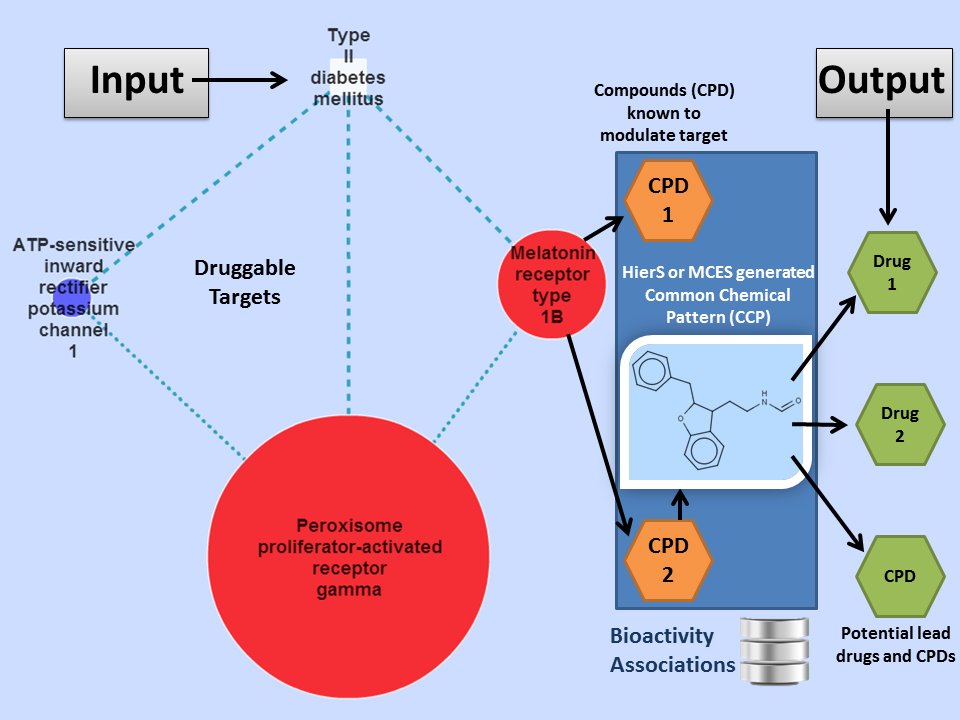
\includegraphics[width=\textwidth]{figures/carlsbad/CB1_Screenshots.png}
    \caption{CARLSBAD schematic}
    \label{fig:cb_schematic}
\end{figure}

Figure 1.
CARLSBAD database entity relationship diagram.

\subsubsection{Data sources, extraction and curation}

Separate extract, transform and load (ETL) pipelines were built for each of the data sources. The sections later in the text detail the specific source of data used and the extraction criteria applied for each.

\textbf{ChEMBL}. A MySQL dump of ChEMBL v13, 2012–02–21 was downloaded from the website and used to create a local MySQL staging database that served as the source from which data were extracted and used to populate the CARLSBAD database (2). ChEMBL data passing the following filters were loaded into CARLSBAD. Only activities from publications were loaded; activities associated with pharmacokinetic, cellular and in vivo assays, and any other activities not associated with a protein target were not imported; activities not associated with human, rat and mouse targets were skipped; and activities without values or units that could be converted to -log(molar) were also skipped. Activities of the following type were loaded: EC50, IC50, pEC50, pIC50, Log EC50, Log IC50, Ki, Kb, Kd, pKi, pKb, pKd, Log Ki, Log Kb, LogKd, ED50, IC80, IC90, A2, D2, pA2, pD2 and Km. Also, activities with units expressed in molarity, as well as activities with an associated structure were loaded. Additionally, activity values were converted to molar wherever necessary and converted to negative log where appropriate.

\textbf{IUPHAR}. Data were programmatically extracted from the IUPHAR website (http://www.iuphar-db.org/) and used to populate a local MySQL staging database. This staging database was constructed during February 2011 and served as the source from which data were extracted and used to populate the CARLSBAD database. Only activities with the following classes were loaded: agonists, antagonists, pore blockers, activators, allosteric regulators, gating inhibitors and channel blockers. In addition, midpoints or medians were used for affinities expressed as ranges. Activities not associated with human, rat and mouse targets as well as activities with unknown affinities or units were excluded.

\textbf{PDSP}. The text file (kidb110121.txt) was downloaded from the website (http://pdsp.med.unc.edu/indexR.html). UniProt IDs were added to this file by the group of Stephan Schurer, University of Miami. This file was used as the source from which data were extracted and used to populate the CARLSBAD database. Only PDSP data passing the following filters were loaded into CARLSBAD. Activities associated with structures not parseable by gNOVA, and activities with qualified values (i.e. \textgreater x) were skipped.

\textbf{PubChem}. Only the subset of PubChem derived from the Molecular Libraries Probe Network (PubChem MLP) was used. The PubChem Assays and Substances to be loaded into CARLSBAD were selected using the Entrez EUtils API to search pcassay with the following queries/filters: ‘Molecular Libraries Probe Production Centers Network[SourceCategory]’, confirmatory[Filter] and pcassay\_protein\_target[Filter]. Substance structures were retrieved as SMILES using the PubChem Power User Gateway (PUG). Assay data were loaded from xml and csv files downloaded from the PubChem ftp site. PubChem MLP data passing all of the following filters were loaded into CARLSBAD. Only activities associated with human, rat or mouse targets were loaded. Only activities with the following result types were loaded: various versions of EC50, AC50, IC50, Ki and Potency. Activities without values or units were skipped. Only activities with units expressed in molarity were loaded. Only activities with an associated structure were loaded. Additionally, activity values were converted to molarity if necessary, and activity values were converted to negative Log10 if necessary.

\textbf{WOMBAT}. Version 2011.2 (SDF and activities.tab files) was used as the source from which data were extracted and used to populate the CARLSBAD database. Only activities of the following types were loaded: EC50, ED50, IC50, IC80, IC90, Ki, Kb, Kd, Km, A2 and D2. In addition, the following data were skipped: activities not associated with a known target; activities not associated with human, rat and mouse targets; activities associated with targets without an associated UniProt identifier; activities from primary screening; activities labeled ‘inactive’; and activities with descriptive values (e.g. ‘active’).

When pairing structures with targets and bioactivities in a similar effort, Tikkainen and Franke observed that only 3.6\% (i.e. 410 of 11,278) of the scientific articles with activity indexed in more than one database matched each other. Indeed, data discrepancies are ubiquitous as far as data curation is concerned\cite{Tiikkainen2012-cw}. The processing log for CARLSBAD is summarized in Table 1: of 975,117 unique structure–target pairs in the database, 84 794 were found unique to WOMBAT and, therefore, have not been processed into CARLSBAD. For the remaining 890 323 structure–target pairs, 124,231 (13.95\%) were aggregated from multiple structure–target values: 94,975 from two bioactivities, 14,544 from three, 7930 from four and 2214 from five bioactivities, respectively. The highest number of consolidated bioactivities is 109, with the second highest number being 106. As data aggregation is the intended purpose for CARLSBAD, we focused on eliminating extremes in the bioactivity spectrum, and aggregating values towards a mean value. Hierarchical processing (i.e. confidence levels) was used in $\sim$25\% of the cases (192,736 + 38,670 substance–target pairs) when generating the CARLSBAD activity.

\begin{table}[]
\centering
\begin{tabular}{c|c}
\hline
\textbf{Processed substance–target pairs} & \textbf{Number of bioactivities} \\
\hline
975,117 & Initial aggregated data   \\
975,110 & Valid processed pairs   \\
84,794 & WOMBAT only   \\
658,917 & Only one activity on record  \\ 
192,736 & Only one activity type (each entered)  \\ 
38,670 & Multiple activity types processed   \\
932,881 & total activities loaded   \\
\hline
\end{tabular}
\caption{CARLSBAD database consolidation process summary}
\label{tab:cb_01}
\end{table}

\subsubsection{Chemical curation}

In the CARLSBAD database, chemical substances are distinguished from compounds in a manner analogous to the PubChem terminology. In this paradigm, compounds represent the abstract structure of any of the components of the substance. Chemical structures are stored as canonical SMILES using CHORD (gNova/OpenEye). The corresponding SDF format is also stored if present in the input database. In addition, 26 chemical descriptors are calculated and stored for each unique compound. These descriptors (e.g. molecular weight, number of rings and so forth) are provided for convenience to users interested in specific subsets of chemical space. A key feature of the CARLSBAD database is the common chemical patterns (CCPs), which are calculated and associated with the corresponding chemical structures. Later in the text, we briefly describe the methods used to calculate the two types of CCPs and how they are stored.

\subsubsection{HierS}

HierS, the hierarchical scaffold grouping algorithm\cite{Wilkens2005-ja} (9), is based on the molecular framework concept described by Bemis and Murcko\cite{Bemis1996-jg}. The ‘scaffold’ concept is central in medicinal chemistry and provides a chemically intuitive manner to visualize chemical classes, as ring-based linkages are central structural features in most (\textgreater 90\%) drug molecules. The algorithm relates any two compounds by their common shared scaffolds. HierS has two advantages: (i) speed and (ii) HierS scaffolds are considered by some to be more meaningful than the typical maximum common substructure (MCS). To our knowledge, there is no currently available implementation of HierS in any commercial or open-source package. These tools are implemented in an open-source Java library (http://code.google.com/p/unm-biocomp-hscaf/) built on the JChem toolkit from ChemAxon.

\subsubsection{MCES}

MCES. The maximum common edge subgraph (MCES) concept\cite{Raymond2002-ep} can be used to compute similarity between two molecular graphs and has been widely used in many applications\cite{Stahl2005-bl,Sheridan2006-nx,Gardiner2007-ur,Bocker2008-uh,Hariharan2011-qx,Bostrom2012-fb}. However, MCES computation is NP complete, and several heuristics have been proposed to reduce computational time, although computational time required for large chemical datasets is prohibitive. Thus, in the CARLSBAD database, additional heuristics based on common ring systems/scaffolds were applied to further reduce computational time and make feasible MCES computation for large libraries. The CARLSBAD database contains 435,578 compounds with \textgreater99\% compounds containing at least one ring. As ring system determination using HierS is efficient and fast, scaffold information determined using HierS was used to group compounds based on the number of common scaffolds shared between them. Once this preliminary heuristic was applied, pairwise MCES between compounds sharing the same set of scaffolds was computed. Thus, the MCES algorithm was run on the CARLSBAD database and used to identify clusters of compounds with shared maximum common substructures.

\subsubsection{Target curation}

Representation of targets varies greatly across source databases, and this creates several challenges. In particular, targets are named and identified in different ways, which makes it difficult to know whether a target from one data source is the same as a target from another source, i.e. target matching and ‘unification’. As the goal was to have one target record in CARLSBAD for each unique protein represented in assays, a target curation step was performed after each data source was loaded, where newly loaded targets were annotated with data from UniProt\cite{UniProt_Consortium2018-kq}, to expedite the target unification process. Targets identified in the source data by SwissProt or UniProt IDs were annotated with name, description, sequence and other identifiers (NCBI gi, RefSeq, Gene, UniGene and PDB) from UniProt. This allowed a comparison for target redundancy by sequence and identifiers after each data source was loaded to be made. Data from UniProt were also used to annotate targets in the CARLSBAD database with the following classifiers: InterPro, Pfam and PROSITE domains; GO terms; and UniProt family.

\subsubsection{Web interface}

A browsing and query interface to the CARLSBAD database is available (http://carlsbad.health.unm.edu/carlsbad/) (Figure 2). This web interface is delivered via the open source Apache web server. The application is written in the Perl programming language and uses Marvin Java applets from ChemAxon for drawing and displaying chemical structures. Users can query from structures by name, structure and/or properties; and for targets by name, species, type and/or identifier.

Figure 2.
CARLSBAD Web Application. (A) Query forms. (B) Activity search results. (C) Substance view.

\subsection{Discussion}

The availability of massive amount of molecular bioactivity data creates rich new opportunities, yet for typical scientists involved in biomedical discovery research, the difficulty of processing and analyzing that data can often be a barrier. With the occasional, less experienced end-user in mind, we have developed a small molecule bioactivity database that facilitates navigation in the small molecule/bioactivity space. The unique features and underlying data structure of the CARLSBAD database are designed to support polypharmacology-driven drug discovery scenarios, such as drug repurposing, side effect/off-target prediction and lead identification workflows.

The net result of chemical, bioactivity and target aggregation, curation and harmonization is summarized in table \ref{tab:cb_02}: the number of substances, i.e. chemicals tested for bioactivity, is smaller than the one obtained by summing the five databases by 17.27\%. A similar trend is observed when examining bioactivities (34.35\% reduction) and CCPs (23.1\% reduction using HierS and 25\% using MCES). The aforementioned values are the result of machine-based harmonization and consolidation of multiple data objects in chemical, bioactivity and CCP space. An independent study by Tiikkainen and Franke\cite{Tiikkainen2013-md,UniProt_Consortium2018-kq}, comparing ChEMBL (release 14) and WOMBAT 2012.01, showed \textgreater 394,000 unique bioactivities in WOMBAT, compared with nearly 3.3 million bioactivities in ChEMBL; and 2755 unique targets in ChEMBL, compared with 1486 unique targets in WOMBAT. The harmonization trends suggest that a consolidated database is preferable to a federated collection, at least in this case, when seeking to evaluate global bioactivity trends. This solution was, for example, implemented in the ‘Merz Virtual Bioactivity Database’, which integrates ChEMBL and WOMBAT, among other data sources.

\begin{table}[]
\caption{Overview of the numbers of substances, activities and CCP data in the original databases, as well as the consolidated CARLSBAD database}
\label{tab:cb_02}
\centering
\begin{tabular}{p{0.25\linewidth}p{0.15\linewidth}p{0.15\linewidth}p{0.15\linewidth}p{0.30\linewidth}}
\hline
\textbf{Source (Version)} & \textbf{Release date} & \textbf{Structures} & \textbf{Activities} & \textbf{CCPs} \\
\hline
ChEMBL (13) & 2012–02–21 & 267,744 & 798,755 & \makecell[l]{182,496 scaf \\ 32,794 mces} \\
IUPHAR & 2011 & 2297 & 6049 & \makecell[l]{2704 scaf \\ 652 mces} \\
PDSP (kidb110121) & & 3499 & 22,202 & \makecell[l]{3422 scaf \\ 823 mces} \\
PubChem (MLP) & 2011–11–04 & 133,435 & 320,311 & \makecell[l]{83,570 scaf \\ 20,867 mces} \\
WOMBAT & 2011.2 & 124,873  & 273,572 & \makecell[l]{88,135 scaf \\ 17,086 mces} \\
Total & & 531,848 & 1,420,889 & \makecell[l]{360,327 scaf \\ 72,222 mces} \\
CARLSBAD & 2012.1 & 439,985 & 932,881 & \makecell[l]{277,140 scaf \\ 54,135 mces} \\
\hline
\end{tabular}
\end{table}

Comparing the databases, it is apparent that ChEMBL is the most populated in terms of substances, bioactivities and CCPs, followed by WOMBAT and PubChem/MLP. This is to be expected, given their chemogenomic purpose. Two of the databases dedicated to pharmacology, IUPHAR and PDSP, are significantly smaller. An in-depth comparison with respect to targets, bioactivities and chemistry coverage for some of these databases has been performed\cite{Tiikkainen2012-cw}. Each of these databases provided relevant contributions in terms of CARLSBAD aggregation.

Chemical errors were addressed with focus on the high-value, high-confidence IUPHAR and PDSP subsets. We found only one PDSP structure that was not parsable by gNova/OEChem; it was manually corrected. For IUPHAR, we extensively curated \textgreater 2700 small molecules and peptides from IUPHAR’s ‘Ligand List’ (http://www.iuphar-db.org/DATABASE/LigandListForward: retrieved fourth February 2011). This curation involved reading the original ligand references to resolve ligand names, 2D structures and biological activities, including \textgreater700 peptides for which structural information was not then available in IUPHAR-DB\cite{Harding2018-ut}. In the future, the teams supporting the CARLSBAD and IUPHAR-DB projects will work together to ensure the consistency of data between the two resources.

When aggregating data in CARLSBAD, we did not explicitly address biology or bioactivity errors. By cross-referencing PubMed IDs for literature-based data (i.e. PDSP, IUPHAR-DB, ChEMBL and WOMBAT), we found that identical articles are covered by these resources, yet data are not always identical. Indeed, up to 3\% errors in target protein identity, up to 2.7\% errors in bioactivity values, and up to 7\% errors in chemical structure depiction were found in comparing three data sources. In CARLSBAD, these tuples were harmonized by providing median values wherever possible, and by representing ‘higher curation’ values where possible, when multiple conflicting values were found. For example, bioactivity results from IUPHAR-DB were given the highest priority, as they summarize the significant curation effort made by members of the IUPHAR Nomenclature Committee. Overall, this situation occurred in \textless 10\% of the database. With respect to data generated by the NIH Molecular Libraries Initiative\cite{Austin2004-qc}, only data from PubChem was uploaded into CARLSBAD, as stated earlier in the text. Thus, any bioactivity value ‘feedback loop’, i.e. propagation of errors from one database to another, was avoided by importing non-overlapping sets of data.

Chemical space overlap between structures in the CARLSBAD database and drugs approved for human use was determined using structure identity comparison with an in-house curated database of drug structures approved worldwide (DRUGSDB), which includes discontinued drugs as well\cite{Oprea2010-kd,Manallack2013-qm}. A total of 1435 unique chemical structures for active pharmaceutical ingredients (i.e. ‘drugs’) were identified in CARLSBAD of $\sim$4000 small organic molecules from DRUGSDB. These chemical structures were flagged accordingly for user convenience and can be used to explore biological activity space of known drugs.

CARLSBAD represents only a first step in our effort to assist non-expert scientists to navigate chemical biology data. For example, all protein targets related to estrogen biology can be identified via a single CARLSBAD query. However, their inter-connectedness via chemicals and CCPs is intended to be explored in the networked environment provided by Cytoscape\cite{Shannon2003-ph}. The CARLSBAD network extraction tool (SNAKE), the Cytoscape plugin and the process of visualizing networks of connected protein targets, chemical structures and bioactivities, are described elsewhere.

\subsection{Summary}

CARLSBAD is a database focused on high-quality subsets aggregated from several bioactivity databases, which are integrated in a uniform interface and manner, suitable for chemical biology and drug discovery studies, as well as large scale, ‘big data’ informatics and knowledge mining. In contrast to the original data collections, CARLSBAD provides a single normalized activity value of a given type for each unique chemical–protein target pair. Aggregation accounted for $\sim$25\% of the \textgreater 975,000 structure–target pairs processed, up to and including 109 bioactivities for a single chemical. CARLSBAD data processing resulted in a net 17.3\% reduction in terms of unique chemicals, 34.3\% reduction in terms of unique bioactivities and \textgreater 23\% reduction in terms of CCPs, respectively, suggesting that data consolidation is preferable to a federated database system, at least where bioactivity is concerned. We implemented two types of scaffold perception for common chemical pattern detection HierS and MCES, respectively. The 2012 release of CARLSBAD contains 439,985 unique chemical structures, mapped onto 1 420,889 unique bioactivities and annotated with 277,140 HierS scaffolds and 54,135 MCES patterns, respectively. It also contains bioactivities and tags for 1435 unique active pharmaceutical ingredients. The CARLSBAD database can be accessed using SNAKE; our dedicated subnet extraction tool, and Cytoscape, via the CARLSBAD plugin (Hines-Kay et al., submitted for publication).




\section{OPDDR: Open phenotypic drug discovery resource}

OPDDR: Open Phenotypic Drug Discovery Resource
Novel Phenotypic Outcomes Identified for a Public Collection of Approved Drugs from a Publicly Accessible Panel of Assays, J. Lee, et al, PLoS ONE, 2015\cite{Lee2015-vg}.

Collaboration involving Lilly's Open Innovation Drug Discovery (OIDD), NIN-NCATS, Data2Discovery and IU.  

My role included converting the dataset to RDF,  annotating assays using BioAssay Ontology (BAO), and coordinating with PubChem and Open PHACTS to deposit assay results and incorporate OPDDR.
Poster: https://zenodo.org/record/4844529

\subsection{Introduction}

This report is submitted in accordance with the Lilly Resarch Collaboration Agreement between Eli Lilly \& Co (Lilly) and Data2Discovery, executed on June 11, 2015.  The work is part of an ongoing collaboration involving Lilly, NIH-NCATS, and Data2Discovery.  The role of Data2Discovery is informatics: transforming and integrating data to enhance semantic value, development of a Knowledge Network (KN), a publicly shared Open Phenotypic Drug Discovery Resource (OPDDR, aka PD2) which can be used to identify relationships between National Pharmaceutical Collection (NPC) compounds, phenotypic assays, ontological classes of assays, and associated public data on related molecular targets.

\subsection{Accomplishments}

As per the agreement, the OPDDR has been developed and deployed, hosted by NCATS. 

The recently and significantly revised (June 2015) PubChem RDF data model was integrated, informed via engagement with PubChem team (Bolton et al.) initiated by Data2Discovery.

BioAssay Ontology (BAO) integration informed by discussions with BAO team (S. Schurer), and with AstraZeneca (O. Enqvist) regarding their assay annotation template. 

OpenPHACTS (OP) integration informed by discussions with OP, which entailed major revisions in the KN, and also revisions in the OP data model and API, to handle phenotypic assays. 

\subsection{Knowledge Network Description}

The initial version of the KN is intended to provide a clear and easily comprehensible first step of describing the OPDDR compounds and assays in accordance with standardized community ontologies and namespaces, and relating these to protein targets from ChEMBL.  Biological networks can be extremely complex, and many further entity classes can be integrated in future (e.g. pathways), and will be facilitated by this initial KN.

\subsubsection{Ontologies Used}

The KN uses the following ontologies:

\begin{table}[]
\caption{Ontologies}
\label{tab:opddr_01}
\centering
\begin{tabular}{p{0.3\linewidth}p{0.7\linewidth}}
\hline
\textbf{PubChem RDF} & Primary reference for this project.  Mainly because assays and substances have been deposited into PubChem. 
\textless http://rdf.ncbi.nlm.nih.gov/pubchem/\textgreater \\
\textbf{BAO} & Bioassay classification.  Initially using a minimal set based on annotation template provided by AstraZeneca.  Only bao\_vocabulary\_assay.owl is required currently.
\textless http://www.bioassayontology.org/bao\#\textgreater \\
\textbf{ChEMBL RDF} & ChEMBL, Reactome, Uniprot endpoint \& downloads available.
CCO = ChEMBL Core Ontology
\textless http://rdf.ebi.ac.uk/terms/chembl\#\textgreater \\
\textbf{OBO} & Open Biological and Biomedical Ontologies \\
\textbf{BFO} &  Basic Formal Ontology \textless http://purl.obolibrary.org/obo/\textgreater \\
\textbf{SIO} & Semanticscience Integrated Ontology
\textless http://semanticscience.org/resource/\textgreater \\
\end{tabular}
\end{table}


\subsubsection{Entities}

\begin{table}[]
\caption{Entities}
\label{tab:opddr_02}
\centering
\begin{tabular}{p{0.3\linewidth}p{0.7\linewidth}}
\hline
\textbf{entity} & \textbf{namespace (example)} \\
\hline
substance & \makecell[l]{\textless http://rdf.ncbi.nlm.nih.gov/pubchem/substance/\textgreater \\ (SID124893119)} \\
compound & \makecell[l]{\textless http://rdf.ncbi.nlm.nih.gov/pubchem/compound/\textgreater \\ (CID1131)} \\
assay & \makecell[l]{\textless http://rdf.ncbi.nlm.nih.gov/pubchem/bioassay/\textgreater \\ (AID1117354)} \\
measuregroup & \makecell[l]{\textless http://rdf.ncbi.nlm.nih.gov/pubchem/measuregroup/\textgreater \\ (AID1117354)} \\
endpoint & \makecell[l]{\textless http://rdf.ncbi.nlm.nih.gov/pubchem/endpoint/\textgreater \\ (SID124893119\_AID1117354)} \\
protein & \makecell[l]{\textless http://rdf.ncbi.nlm.nih.gov/pubchem/protein/\textgreater \\ (GI124375976)} \\
target & \makecell[l]{\textless http://rdf.ebi.ac.uk/resource/chembl/target/\textgreater \\ (CHEMBL3038470)} \\
targetcomponent & \makecell[l]{\textless http://rdf.ebi.ac.uk/resource/chembl/targetcomponent/\textgreater \\ (CHEMBL\_TC\_1927)} \\
UniprotRef & \makecell[l]{\textless http://rdf.ebi.ac.uk/terms/chembl\#UniprotRef\textgreater \\ (P53350)} \\
assay & \makecell[l]{\textless http://rdf.ebi.ac.uk/resource/chembl/assay/\textgreater \\ (CHEMBL987214)} \\
activity & \makecell[l]{\textless http://rdf.ebi.ac.uk/resource/chembl/activity/\textgreater \\ (CHEMBL\_ACT\_2470294)} \\
molecule & \makecell[l]{\textless http://rdf.ebi.ac.uk/resource/chembl/molecule/\textgreater \\ (CHEMBL44884)} \\
\hline
\end{tabular}
\end{table}

Note that PubChem compounds are required in addition to substances.  Compounds refer to canonically defined and identifiable chemical entities which can be linked across databases; Substances refer to specific samples of compounds as provided by a supplier.  We thus include both, to be as comprehensive and specific as possible.   Note also that PubChem measuregroups are defined for each assay, for example, the measuregroup URI for AID12345 is http://rdf.ncbi.nlm.nih.gov/pubchem/measuregroup/AID12345.  PubChem endpoints represent activity outcomes.  ChEMBL RDF represents bioactivities somewhat differently than PubChem, but we can rigorously link these data via chemical structure and CIDs.

\begin{table}[]
\caption{KN Statistics}
\label{tab:opddr_03}
\centering
\begin{tabular}{p{0.3\linewidth}p{0.2\linewidth}p{0.5\linewidth}}
\hline
\textbf{type} & \textbf{count} & \textbf{notes} \\
\hline
substance & 2511 & PubChem SIDs \\
compound & 2511 & PubChem CIDs \\
assay & 35 & PubChem AIDs.  Summary AID is 36th. \\
measuregroup & 35 & PubChem AIDs.  Default for assay. \\
endpoint & 2511*35 & PubChem SID-AID pairs. \\
targets & 4977 & ChEMBL IDs.  All single-component. \\
protein & 4977 & A.k.a. target component.  With UniprotRefs. \\
protein activity & 584,157 & From ChEMBL, but includes PubChem data. \\
PD2 activity & 5320 & All “ACTIVE” outcomes from results. \\
assay classifications & 155 & Manually curated PD2 to BAO associations.  Exported from worksheet. \\
\hline
\end{tabular}
\end{table}

\begin{table}[]
\caption{Asserted triplets, patterns and examples }
\label{tab:opddr_04}
\centering
\begin{tabular}{p{0.3\linewidth}p{0.7\linewidth}}
\hline
\textbf{description} & \textbf{examples} \\
\hline
assay to BAO class & bioassay:AID1117354 rdf:type bao:BAO\_0000015 \\
assay title & bioassay:AID1117354 dcterms:title "human JAK2 kinase inhibition-screen"@en \\
assay to measuregroup & bioassay:AID1117354 bao:BAO\_0000209 measuregroup:AID1117354 \\
substance to NCGC ID & substance:SID144206486 skos:exactMatch ncats\_sample:NCGC00182710-02 . \\
substance to measure group & substance:SID124882766 obo:BFO\_0000056 measureg:AID1117326 \\
endpoint outcome (activity) & endpoint:SID170466632\_AID743241 vocabulary:PubChemAssayOutcome vocabulary:inactive \\
endpoint class & endpoint:SID103164874\_AID443491 rdf:type bao:BAO\_0000190 \\
substance to compound association & substance:SID124893119 sio:CHEMINF\_000477 compound:CID1131 \\
assay to OIDD ID & bioassay:AID1117350 skos:exactMatch  oidd\_assay:17 \\
ChEMBL target to UniProt & chembl\_target:CHEMBL5464 cco:targetXref uniprot:Q13546 \\
ChEMBL target to assay & chembl\_target:CHEMBL5464 cco:hasAssay assay:CHEMBL3110727 \\
ChEMBL target to target component & chembl\_target:CHEMBL1867 cco:hasTargetComponent chembl\_targetcmpt:CHEMBL\_TC\_180 \\
ChEMBL target component to Uniprot & chembl\_targetcmpt:CHEMBL\_TC\_180 cco:targetCmptXref uniprot:P08913 \\
ChEMBL assay to activity & assay:CHEMBL3110727 cco:hasActivity activity:CHEMBL\_ACT\_13890030 \\
ChEMBL molecule to activity & chembl\_molecule:CHEMBL313842 cco:hasActivity activity:CHEMBL\_ACT\_14447741 \\
PubChem substance to ChEMBL molecule & substance:SID225144242 skos:exactMatch molecule:CHEMBL1474122  \\
\hline
\end{tabular}
\end{table}

Fig: OPDDR RDF schema, simplified, showing source relationships.

\subsubsection{Files}

\begin{table}[]
\caption{The following files comprise this release.  Files are grouped below by source, each file from one source only.}
\label{tab:opddr_05}
\centering
\begin{tabular}{p{0.3\linewidth}p{0.7\linewidth}}
\hline
\textbf{file (source)} & \textbf{description} \\
\hline
npcpd2\_assay.ttl (OPDDR) & Assay links to OIDD namespace. 
bioassay:AID1117326 skos:exactMatch oidd\_assay:4 \\
npcpd2\_bao.ttl (OPDDR) & Manually curated BAO classifications. 
bioassay:AID1117352 rdf:type bao:BAO\_0000219 \\
npcpd2\_substance.ttl (OPDDR) & Substance links to NCATS namespace. 
substance:SID170465644 skos:exactMatch ncats\_sample:NCGC00160518-03 \\
bao\_vocabulary\_assay.owl (BAO) & BAO module with bioassay class hierarchy.  \\
pubchem\_vocabulary.owl (PubChem) & PubChem module with bioactivity terms etc. \\
pubchem\_pd2\_assay.ttl (PubChem) & PubChem RDF, includes titles, measuregroups. 
bioassay:AID1117356 bao:BAO\_0000209 measuregroup:AID1117356 
bioassay:AID1117351 dcterms:title "Increased HeLa cells with 4N DNA content-IC50"@en  \\
pubchem\_pd2\_substance.ttl (PubChem) & PubChem RDF, includes CIDs, measuregroups. 
substance:SID124882766 obo:BFO\_0000056 measuregroup:AID1117326 . 
endpoint:SID124882766\_AID1117342 obo:IAO\_0000136 substance:SID124882766 . \\
pubchem\_pd2\_endpoint.ttl (PubChem) & PubChem RDF, includes endpoints, activity results.
endpoint:SID170464708\_AID1117354 
    obo:IAO\_0000136 substance:SID170464708 ; 
    vocabulary:PubChemAssayOutcome vocabulary:inactive . 
measuregroup:AID1117354 obo:OBI\_0000299 endpoint:SID170464708\_AID1117354 . \\
chembl\_cco.ttl (ChEMBL) ChEMBL Core Ontology \\
chembl\_target.ttl (ChEMBL) & ChEMBL protein targets. 
chembl\_target:CHEMBL2366239 a cco:SingleProtein ; dcterms:title "KLE" \\
chembl\_rdf\_activity.ttl (ChEMBL) & \makecell{PubChem substance links to ChEMBL molecules, activities, assays, targets, target components, Uniprots. \\ substance:SID170466134 skos:exactMatch chembl\_molecule:CHEMBL1230222 \\ chembl\_molecule:CHEMBL44884 cco:hasActivity chembl\_activity:CHEMBL\_ACT\_7667167 . \\ chembl\_target:CHEMBL218 cco:hasAssay chembl\_assay:CHEMBL1909122 . \\ chembl\_target:CHEMBL218 cco:hasTargetComponent chembl\_targetcmpt:CHEMBL\_TC\_172 . \\ chembl\_targetcmpt:CHEMBL\_TC\_172 cco:targetCmptXref uniprot:P21554 . \\ uniprot:P21554 a cco:UniprotRef . } \\
\hline
\end{tabular}
\end{table}


\subsection{Project Status, Future}

This initial KN Beta Version provides sufficient associations for semantic exploration across PD2 phenotypic and public biochemical assays for the NPC substances.  The integration with PubChem, ChEMBL, and OpenPHACTS adds value in multiple ways, linking to a large, diverse and expanding ecosystem of public biomedical knowledge.  Additional assay annotations can add further value, whereby the knowledge model developed can represent and derive high value from the unique knowledge of domain specialists and facilitate the links which power and advance data intensive research.



\section{TIN-X: Target importance and novelty explorer}

TIN-X: Target importance and novelty explorer
TIN-X: Target Importance and Novelty Explorer, D.C. Cannon et al., Bioinformatics, 2017\cite{Cannon2017-af}.

Estimates and visualizes the association between proteins and diseases, based on text mining data processed from scientific literature.  Novelty estimates the scarcity of publications about a protein target. Importance estimates the strength of the association between that protein target and a specific disease.
Web application: https://newdrugtargets.org
Poster: https://zenodo.org/record/5038628

\subsection{Abstract}

Summary: The increasing amount of peer-reviewed manuscripts requires the development of specific mining tools to facilitate the visual exploration of evidence linking diseases and proteins. We developed TIN-X, the Target Importance and Novelty eXplorer, to visualize the association between proteins and diseases, based on text mining data processed from scientific literature. In the current implementation, TIN-X supports exploration of data for G-protein coupled receptors, kinases, ion channels, and nuclear receptors. TIN-X supports browsing and navigating across proteins and diseases based on ontology classes, and displays a scatter plot with two proposed new bibliometric statistics: Importance and Novelty. 
Availability  and implementation:  available at http://www.newdrugtargets.org/

\subsection{Introduction}

Science builds upon past discoveries, traditionally communicated through words and symbols assembled into works of (peer-reviewed) scientific literature. However, scale-out of traditional and alternate publication modes has exceeded the limit of how much the human mind can process, creating the need for computer-assisted methods\cite{Hunter2006-om}. Text mining, ontologies, and interactive visualization are some of the emerging technologies that can alleviate information overload. We present a new method and software tool utilizing these technologies, to provide biomedical scientists with rankings and visualizations linking proteins and diseases.  The information is derived from PubMed abstracts, text mined using previously published tools for named entity recognition (NER) of gene/protein and disease names\cite{Pletscher-Frankild2015-oo,Szklarczyk2015-bl}. We propose two new bibliometric indices based on NER mentions, specifically devised to address research planning use cases. Our goal is to enable scientists to identify research subjects with sufficient evidence of importance, but not already well-studied. Novelty measures the scarcity of publications about a protein target (see also equation \ref{eq:tinx_n}). Importance measures the strength of the association between that target and a disease (see also equation \ref{eq:tinx_i}). By visualizing Novelty and Importance on a 2D plot, users can easily examine the strength of the evidence linking protein targets and diseases of interest. TIN-X is a web application which allows users to navigate targets via the Drug Target Ontology (DTO, http://drugtargetontology.org) and diseases via the Disease Ontology (DO)\cite{Kibbe2015-li}, and for selected classes, to display and browse Importance–Novelty plots. These plots are interactive, with built-in drill-down and link-out functionality for in-depth examination of selected targets. TIN-X was inspired by and developed for the Illuminating the Druggable Genome (IDG) Knowledge Management Center (KMC, http://targetcentral.ws), which seeks to identify and prioritize understudied genes and proteins for investigation and validation as new drug targets.

\subsection{Methods and Implementation}

The TIN-X web application is implemented in Scala using the Lift web framework (http://liftweb.net), which provides inherent scalability and compatibility with Java.  The back-end utilizes a PostgreSQL database built using the knowledge base developed by the IDG-KMC, and known as the Target Central Research Database (TCRD)\cite{Nguyen2017-lo}.  TCRD compiles data from a variety of sources, including Disease Ontology, and, by special arrangement with IDG-KMC network members, (1) U. Miami, developers of DTO, and (2) NNFCPR, mapping to genes/proteins and diseases using a highly efficient dictionary-based named entity recognition engine\cite{Pafilis2013-ml} with dictionaries from the STRING\cite{Szklarczyk2015-bl} and DISEASES\cite{Pletscher-Frankild2015-oo} databases, respectively.  Data is transferred, processed, and loaded into TCRD by automated and semi-automated protocols, with routine updates approximately bi-annually.  PubMed abstracts are obtained via NCBI web services.  Bibliometric statistics and the derived novelty ($N_i$) and importance ($I_{ij}$) scores are pre-computed for runtime performance, using equations \ref{eq:tinx_n} and \ref{eq:tinx_i}.

\begin{equation}
N_i = \frac{1}{\sum_{k}^{}\frac{1}{T_k}}
\label{eq:tinx_n}
\end{equation}

\begin{equation}
I_{ij} = \sum_{k}^{}\frac{1}{T_kD_k}
\label{eq:tinx_i}
\end{equation}

where $T_k$ and $D_k$ are the numbers of targets and diseases in abstract k, respectively, and summation over all publications including target (i), and for importance, also including disease (j). Fractional counts are employed to reflect strength of association.  E.g. if a paper mentions three targets, each receives a fractional count $\frac{1}{T} = \frac{1}{3}$.

\subsection{Application Example}

In Figure 1, TIN-X displays targets for a selected disease class, "lung cancer".  The DO hierarchy is navigated in the left panel, and the targets are plotted with log-log Importance-Novelty axes. Searching by disease name and by target name (with auto-suggest) is supported. In the current layout, targets with stronger associations are in the upper part of the plot, while targets with a higher number of publications are on the left side of the plot. In general, more interesting associations will be on the upper right boundary of the plot, where data points represent non-dominated solutions to the multi-objective optimization maximizing both Importance and Novelty.  Targets can be filtered based on Target Development Level, with Tclin representing mode-of-action drug targets\cite{Santos2017-sd}, and Tdark representing the understudied proteins\cite{Nguyen2017-lo}. Targets can also be filtered by protein superfamily, which are currently limited to kinases, ion channels, G-protein coupled receptors (olfactory or not), and nuclear receptors, respectively. In the Fig. 1 example, the target shown is "Potassium voltage-gated channel subfamily H member 4" (KCNH4), which links to 11 articles relevant in lung cancer.  In addition to titles and citations, clicking on each article reveals full abstracts and links out to the complete PubMed record. 

Figure 1. Screenshot of TIN-X.

\subsection{Conclusions and Future Directions}

TIN-X provides an intuitive visualization, ranking, and prioritization platform for scientists interested in potentially novel drug targets, and exploring the relationship between diseases, disease categories, proteins and protein classes, using literature mining.  As with all current text mining, TIN-X cannot replace expert human readers and curators, yet, it is increasingly clear that automated bibliometry is essential given the volume of literature to be processed.  TIN-X is an important interactive tool in the IDG project, and future plans include adding functionality relating to known drugs and drug classes, and inclusion of additional protein classes. More information about Tclin, Tdark and other target development levels can be found at http://www.nature.com/nrd/posters/druggablegenome/nrd\_druggablegenome.pdf
